%{{{ Formatierung

\documentclass[a4paper,12pt]{article}

\usepackage{physics_notetaking}

%%% dark red
%\definecolor{bg}{RGB}{60,47,47}
%\definecolor{fg}{RGB}{255,244,230}
%%% space grey
%\definecolor{bg}{RGB}{46,52,64}
%\definecolor{fg}{RGB}{216,222,233}
%%% purple
%\definecolor{bg}{RGB}{69,0,128}
%\definecolor{fg}{RGB}{237,237,222}
%\pagecolor{bg}
%\color{fg}

\newcommand{\td}{\,\text{d}}
\newcommand{\RN}[1]{\uppercase\expandafter{\romannumeral#1}}
\newcommand{\zz}{\mathrm{Z\kern-.3em\raise-0.5ex\hbox{Z} }}

\newcommand\inlineeqno{\stepcounter{equation}\ {(\theequation)}}
\newcommand\inlineeqnoa{(\theequation.\text{a})}
\newcommand\inlineeqnob{(\theequation.\text{b})}
\newcommand\inlineeqnoc{(\theequation.\text{c})}

\newcommand\inlineeqnowo{\stepcounter{equation}\ {(\theequation)}}
\newcommand\inlineeqnowoa{\theequation.\text{a}}
\newcommand\inlineeqnowob{\theequation.\text{b}}
\newcommand\inlineeqnowoc{\theequation.\text{c}}

\renewcommand{\refname}{Source}
\renewcommand{\sfdefault}{phv}
%\renewcommand*\contentsname{Contents}

\pagestyle{fancy}

\sloppy

\numberwithin{equation}{section}

%}}}

\begin{document}

%{{{ Titelseite

\title{Praktikumsversuche}
\author{Jonas Wortmann}
\maketitle
\pagenumbering{gobble}

%}}}

\newpage

%{{{ Inhaltsverzeichnis

\fancyhead[L]{\thepage}
\fancyfoot[C]{}
\pagenumbering{arabic}

\tableofcontents

%}}}

\newpage

%{{{

\fancyhead[R]{\leftmark\\\rightmark}

%{{{ 102
\section{102: Freie und erzwungene Schwingung mit Dämpfung}
In diesem Versuch sollen die grundlegenen Gesetzmäßigkeiten der mechanischen Schwingung anhand des \textsc{Pohl}'schen Drehpendel untersucht werden.\\\\
\textbf{Theorie} 
\begin{enumerate}[label=--]
        \item Wirbelstrombremse \hspace{25pt}
                Ein leitender Drehkörper bewegt sich durch einen Luftspalt in einem Elektromagneten, dessen Feldstärke variabel ist. 
                Aufgrund der Bewegung des Drehkörpers erfahren die Elektronen im Drehkörper ein zeitlich veränderliches Induktionsfeld, wodurch ein elektrische Rotationsfeld aufgebaut wird. 
                Dieses Rotationsfeld erzeugt ein dem Elektromagneten entgegengerichtetes Magnetfeld (\textsc{Lenz}'sche Regel), welches die Pendelbewegung bremst.
        \item Resonanz \hspace{25pt} 
                Resonanz bezeichnet die Fähigkeit eines Systems, seine Amplitude in Abhängigkeit einer Erregerfrequenz zu erhöhen.
                Ist die Dämpfung des Systems bei $\delta =0$, so kommt es für ein Verhältnis von Erreger-- und Eigenfrequenz von 1 zur Resonanzkatastrophe.
\end{enumerate}
\textbf{Messungen} 
\begin{enumerate}[label=--]
        \item Eigenfrequenz \hspace{25pt} 
                Die Eigenfrequenz wird mit der Schwingungsdauer bei abgeschalteter Wirbelstrombremse und abgeschaltetem Motor bestimmt.
                \begin{align} 
                        \nu _0=\tfrac{1}{T}
                .\end{align} 
        \item Güte \hspace{25pt} 
                Das Verhältnis gespeicherter Energie zum thermischen Energieverlust während der folgenden Schwingung.
                Zur Bestimmung kann das Verhältnis der Frequenz der relativen Maximalamplitude, zum Abstand der beiden Frequenzen bei denen die relative Amplitude auf das $2^{-1/2}$--fache abgefallen ist verwendet werden.
                \begin{align} 
                        Q=\dfrac{\nu _{\text{max} }}{\Delta \nu }
                .\end{align} 
                Die Güte kann auch über eine Dämpfung bestimmt werden. Mit abklingenden Amplituden $\varphi _n\left(t\right)=\varphi _0\text{e}^{-\beta nT}$ folgt 
                \begin{align} 
                        \ln \varphi _n=\ln \varphi _0-\beta Tn
                .\end{align} 
                Trägt man $\varphi $ gegen $n$ auf folgt aus der Steigung
                \begin{align} 
                        \dfrac{\Delta \ln \varphi _n}{\Delta n}=-\beta T=:-\ln K
                ,\end{align} 
                folgt das Dämpfungsverhältnis $K$ und die Güte $Q=\tfrac{\pi }{\beta T}$.
        \item Resonanzkurve \hspace{25pt} 
                Die Resonanzkurve kann durch Auftragen der Amplitude des schwingfähigen Systems gegen die Erregerfrequenz bestimmt werden.
\end{enumerate}
%}}}

%{{{ 104
\newpage
\section{104: Physisches Pendel}
In diesem Versuch soll das Trägheitsmoment anhand eines physischen Pendels untersucht werden.\\\\
\textbf{Theorie} 
\begin{enumerate}[label=--]
        \item Trägheitsmoment \hspace{25pt} 
                Das Trägheitsmoment beschreibt die Trägheit einer Masse bei Rotation.
                Für eine Scheibe ist es
                \begin{align} 
                        \Theta =\dfrac{1}{2}mr^2
                .\end{align} 
                In diesem Versuch ist die Pendeldauer der Scheibe gegeben durch
                \begin{align} 
                        T^2=4\pi ^2\dfrac{\Theta }{D}=\left(\dfrac{2\pi }{\omega _0}\right)^2
                ,\end{align} 
                mit $D$ der Richtkonstante des durch die Erdanziehung verursachten Drehmoments. 
                Es gilt
                \begin{align} 
                        M=-D\varphi \approx -amg\varphi \approx -amg\sin \varphi 
                ,\end{align} 
                mit $a$ der Verschiebung der Rotationsachse. 
        \item \textsc{Steiner}'scher Satz \hspace{25pt} 
                Verschiebt sich die Rotationsachse parallel zur ursprünglichen Rotationsache um den Abstand $a$, dann gilt für das gesamte Drehmoment
                \begin{align} 
                        \Theta '=\Theta +ma^2
                .\end{align} 
\end{enumerate}
\textbf{Messung} 
\begin{enumerate}[label=--]
        \item Trägt man $aT^2$ gegen $a^2$ mit Hilfe von
                \begin{align} 
                        aT^2=\dfrac{4\pi ^2\Theta }{mg}+\dfrac{4\pi ^2}{g}a^2
                \end{align} 
                auf, folgt aus der Steigung $\tfrac{4\pi ^2}{g}$.
                Die Amplitude darf hier nur wenige Grad betragen, da sonst keine Kleinwinkelnäherung mehr gilt.
\end{enumerate}
%}}}

%{{{ 106
\newpage
\section{106: Trägheitsmoment}
In diesem Versuch soll das Trägheitsmoment eines Rades anhand der Erhaltungssätze der Mechanik bestimmt werden.\\\\
\textbf{Messung} 
\begin{enumerate}[label=--]
        \item Trägheitsmoment aus Energieerhaltung \hspace{25pt} 
                Aus der Energieerhaltung
                \begin{align} 
                        mgh=\dfrac{1}{2}\left[mv^2+\Theta \omega ^2\right]=\dfrac{1}{2}\left[mr^2+\Theta \right]\omega ^2
                ,\end{align} 
                mit $r$ dem Radius (der Stelle an der der Faden befestigt ist) und $\Theta $ dem Trägheitsmoment des sich drehenden Rades und $m$ der aus Höhe $h$ fallenden Masse, folgt unmittelbar das Trägheitsmoment.
                Für die Auswertung wird $h$ gegen $\omega ^2$ aufgetragen.
        \item Trägheitsmoment aus Impulserhaltung \hspace{25pt} 
                Aus
                \begin{align} 
                        M=\dot{L}
                \end{align} 
                folgt
                \begin{align} 
                        rmg\cdot t = \left[\Theta +mr^2\right]\omega 
                ,\end{align} 
                mit $\Theta $ dem Trägheitsmoment und $r$ dem Radius (der Stelle an der der Faden befestigt ist) des Rades und $m$ der fallenden Masse.
                Für die Auswertung wird $t$ gegen $\omega $ aufgetragen.
        \item Winkelgeschwindigkeit \hspace{25pt} 
                Die Winkelgeschwindigkeit berechnet sich aus
                \begin{align} 
                        \omega =\dfrac{2\pi }{T_1}
                ,\end{align} 
                wobei $T_1$ die Umlaufzeit für einen Umlauf ist. 
                Sie berechnet sich aus $T_1=T/n$ mit $n$ Umläufen. 
                Nachdem die Masse auf dem Boden angekommen ist wird Zeit $T$ und $n$ des noch rotierenden Rades gemessen.
\end{enumerate}
%}}}

%{{{ 108
\newpage
\section{108: Elastizitätskonstanten, Biegung und Knickung}
In diesem Versuch sollen Elastizitätsmodul und Knicklast verschiedener Metalle und Schubmodul eines Torsionsdrahts bestimmt wreden.\\\\
\textbf{Theorie} 
\begin{enumerate}[label=--]
        \item Neutrale Faser \hspace{25pt} 
                Durch den Schwerpunkt einer unter Kraft deformierten Fläche verläuft die der Kraft entsprechenden neutrale Faser, die ihre Länge bei dieser Kraft nicht ändert.
                Die Faser wird allerdings gekrümmt um den Radius $\rho $. 
                Für ein Balkenstück im Abstand $y$ zur neutralen Faser ist die Dehnung
                \begin{align} 
                        \varepsilon =\dfrac{\left(y+\rho \right)-\rho }{\rho }=\dfrac{y}{\rho }
                .\end{align} 
                Die damit einhergehende Zug-- oder Druckspannung folgt aus dem \textsc{Hook}'schen Gesetz
                \begin{align} 
                        \sigma =E\varepsilon =E\dfrac{y}{\rho }
                ,\end{align} 
                mit $E$ dem Elastizitätsmodul.
                Die in die Querschnitte zu übertragenden Drehmomente um den Durchstoßpunkt der neutralen Faser sind gegeben durch
                \begin{align} 
                        M=\iint\sigma y\td y\td x=\dfrac{E}{\rho }\iint_{}^{}y^2\td y\td x\equiv \dfrac{EI}{\rho }
                ,\end{align} 
                mit $I$ dem Flächenträgheitsmoment.
        \item Elastische Linie \hspace{25pt} 
                Die elastische Linie beschreibt die Kurve der neutralen Faser. 
                Es gilt
                \begin{align} 
                        \dfrac{1}{\rho \left(z\right)}=\dfrac{w''\left(z\right)}{\left(1+w'^2\left(z\right)\right)^{3/2}}
                .\end{align} 
                Für kleine Verbiegungen ist $w'^2\left(z\right)\ll 1$. 
                Es gilt dann in erster Näherung
                \begin{align} 
                        w''\left(z\right)=\dfrac{M\left(z\right)}{EI}
                .\end{align} 
                Das Drehmoment ist $M\left(z\right)=F\cdot \left(l-z\right)$. 
                Aus den Anfangsbedingungen $w\left(0\right)=w'\left(0\right)=0$ folgt dann
                \begin{align} 
                        w\left(z\right)=\dfrac{F}{EI}\left(\dfrac{lz^2}{2}-\dfrac{z^3}{6}\right)
                .\end{align} 
                Die maximale Strecke der Biegung ist am Balkenrand bei $z=l$, mit $c=\tfrac{F}{EI}\tfrac{l^3}{3}$.
        \item Knicklast \hspace{25pt} 
                Hier wird ein senkrecht gelagerter bereits ausgelenkter Stab betrachtet.
                Aus der DGL der elastischen Linie
                \begin{align} 
                        w''\left(z\right)+\dfrac{F_0}{EI}w\left(z\right)=0
                ,\end{align} 
                folgt mit den Anfangsbedingungen $w\left(0\right)=w\left(l\right)=0$ die Knicklast
                \begin{align} 
                        F_0=EI\dfrac{\pi ^2}{l^2}
                .\end{align} 
        \item Schubmodul \hspace{25pt} 
                Die Theorie für den Drehschwinger ist analog zu 104.
                Aus der Richtkonstante folgt das Schubmodul $G$ mit
                \begin{align} 
                        D=2\left(\dfrac{\pi }{2}\dfrac{r^4}{l}G\right)
                .\end{align} 
                Die Richtkonstante bestimmt man über den Geradenfit von $T^2$ gegen $a^2$ 
                \begin{align} 
                        T^2=\dfrac{4\pi ^2\left(\Theta _{\text{Stange}}+\Theta _{\text{Zusatzmasse}}\right)}{D}+\dfrac{8\pi ^2m}{D}a^2
                .\end{align} 
\end{enumerate}
\textbf{Messung}
\begin{enumerate}[label=--]
        \item Knicklast \hspace{25pt} 
                Um die Knicklast zu messen werden verschiedene Stäbe vertikal eingespannt und mit Gewichten von oben belastet.
                Die Auslenkung wird gegen die aufgelegte Kraft aufgetragen. 
                Die Knicklast ist an der Stelle, an der die Auslenkung stark ansteigt.
        \item Elastizitätsmodul \hspace{25pt} 
                Das Elastizitätsmodul kann aus der Steigung der Geraden bestimmt werden, wenn Auslenkung gegen Kraft aufgetragen wird.
\end{enumerate}
%}}}

%{{{ 110
\newpage
\section{110: Spezifische Wärmekapazität -- Adiabatenexponent von Luft}
In diesem Versuch werden die spezifischen Wärmekapazitäten von Metallen bestimmt, die \textsc{Dulong}--\textsc{Petit}'sche Regel bestätigt und der Adiabatenexponent von Luft bestimmt.\\
\textbf{Theorie} 
\begin{enumerate}[label=--]
        \item Wärme \hspace{25pt} 
                Die Wärme oder Wärmemenge ist der Teil der Energie der von einem thermodynamischen System aufgenommen oder Abgegeben wird.
                Sie ist näherungsweise
                \begin{align} 
                        Q=C\left(T_2-T_1\right)
                .\end{align} 
                Tauschen zwei Körper mit verschiedenen Temperaturen Energie aus, bis sie die gleiche Endtemperatur $T_=$ haben, gilt
                \begin{align} 
                        C\left(T_1-T_=\right)=C'\left(T_=-T_1'\right)
                .\end{align} 
        \item Wärmekapazität \hspace{25pt} 
                Die Wärmekapazität ist die Proportionalitätskonstante der Wärme.
                Sie ist proportional zur Masse oder Stoffmenge
                \begin{align} 
                        C=c _{\text{spez.}}m=c _{\text{mol.}}n
                .\end{align} 
                Die molare Wärmekapazität von (fast) idealen Gasen und Flüssigkeiten ist
                \begin{align} 
                        c _{\text{mol.}}=\dfrac{1}{2}fR
                .\end{align} 
                Näherungsweise für einen kleinen Temperaturbereich ist die Wärmekapazität von Festkörpern (mit $f=6$) gegeben durch die \textsc{Dulong}--\textsc{Petit}'sche Regel
                \begin{align} 
                        c _{\text{mol.}}=3R
                .\end{align} 
        \item Adiabatenkoeffizient \hspace{25pt} 
                Der Adiabatenkoeffizient ist definiert als 
                \begin{align} 
                        \kappa :=\dfrac{C_p}{C_V}
                ,\end{align} 
                mit ${}_p$ unter isobarer und ${}_V$ unter isochorer Temperaturänderung.
                Der Adiabatenkoeffizient findet sich in der Adiabatengleichung wieder
                \begin{align} 
                        p_1V_1^\kappa =p_2V_2^\kappa =\text{const.}
                .\end{align} 
\end{enumerate}
\textbf{Messungen} 
\begin{enumerate}[label=--]
        \item Wärmekapazität \hspace{25pt} 
                Die Wärmekapazität lässt sich mit einem Wasserkalorimeter bestimmen. 
                Dafür wird eine Masse in einen mit Wasser gefüllten Messingbecher gegeben und gewartet bis sich die Temperatur von Masse und Wasser + Messingbecher ausgeglichen haben. 
                Mit den gemessenen Ausgangstemperaturen und bekannter Wärmekapazität von Wasser und Messing lässt sich dann die Wärmekapazität der Masse bestimmen.\par
                Da der Wärmeaustausch nicht instantan ist und zudem Wärme an die Umgebung verloren geht wird die theoretische Ausgleichstemperatur nicht erreicht.
                Der theoretische instantane Temperaturausgleich lässt sich simulieren, indem eine senkrechte Linie durch den Punkt der größten Steigung gezeichnet wird und die Temperatur des Kalorimeters und die Ausgleichstemperatur an den Schnittstellen mit der Vor-- bzw.\ Nachkurve abgelesen werden.
        \item Adiabatenkoeffizient \hspace{25pt} 
                Der Adiabatenkoeffizient kann mit Hilfe einer freien Schwingung berechnet werden.
                Dafür wird ein Gefäß mit einem Gas gefüllt und an einer langen zylinderförmigen Öffnung mit einem frei Beweglichen Korken aus Metall \glqq verschlossen\grqq{}.
                Unter konstanter Gaszufuhr (Kraft nach außen) und der Gewichtskraft (Kraft nach innen) kann der Korken zu einer freien angeregten Schwingung gebracht werden.
                Diese Schwingung besteht darin, dass der Korken von dem einströmenden Gas aus dem Gefäß herausgedrückt wird, das Gas oben entweicht und der Korken dadruch wieder in das Gefäß fällt, bis genug Druck vom Gas vorhanden ist, um den Korken wieder herauszudrücken.
                Geht man vom Gleichgewicht aus gilt folgende Gleichung
                \begin{align} 
                        p_0=p _{\text{Gas}}=p _{\text{Luft}}+p _{\text{Gewichtskraft}}=p_L+\dfrac{mg}{\pi r^2}
                .\end{align} 
                Hieraus und aus der Adiabatengleichung (der Schwingvorgang verläuft so schnell, dass er quasi adiabatisch ist) kann die DGL des schwingfähigen System aufgestellt werden
                \begin{align} 
                        \ddot{x}+\underbrace{\dfrac{\pi ^2r^4p_0\kappa }{mV_0}}_{=\omega _0^2}x=0
                .\end{align} 
                Mit $T=\tfrac{2\pi }{\omega _0}$ folgt für den Adiabatenkoeffizient
                \begin{align} 
                        \kappa =\dfrac{4mV_0}{T^2r^4p_0}
                .\end{align} 
\end{enumerate}
%}}}

%{{{ 112
\newpage
\section{112: Wärmeausdehnung von Festkörpern}
In diesem Versuch werden Wärmeausdehnungskoeffizienten von verschiedenen Metallen experimentell bestimmt.\\\\
\textbf{Theorie} 
\begin{enumerate}[label=--]
        \item Ausdehnung von Festkörpern \hspace{25pt} 
                Ein Festkörper dehnt sich aus, da auf Grund von Temperaturzufuhr die kinetische Energie der Atome erhöht wird. Die Erhöhung von kinetischer Energie äußert sich in einer größeren Amplitude der Gitterschwingung. 
                Da das \textsc{Lennard-Jonas}--Potential asymmetrisch ist, erhöht sich der über die Schwingungsbewegung gemittelte Abstand der Atome.
        \item Längenänderung \hspace{25pt} 
                Die Längenänderung von Festkörpern bei einer Temperaturänderung $\Delta T$ lässt sich näherungsweise beschreiben durch
                \begin{align} 
                        l=l_0+\Delta l \approx l_0+l_0\alpha \Delta T=l_0\left(1+\alpha \Delta T\right)
                ,\end{align} 
                mit $\alpha $ dem Wärmeausdehnungskoeffizient (einer Materialeigenschaft).
\end{enumerate}
\textbf{Messungen} 
\begin{enumerate}[label=--]
        \item Wärmeausdehnungskoeffizient \hspace{25pt} 
                Dünne Rohre aus verschiedenen Materialien werden von sich erwärmenden Wasser durchflossen, wodurch sich die Rohre näherungsweise immer mit dem Wasser im thermischen Gleichgewicht befinden.
                Zur Auswertung kann $l$ gegen $\Delta T$ aufgetragen werden.
\end{enumerate}
%}}}

% todo 232 Messungen? Was soll da so gemessen werden? Was ist wichtig?
% todo 234 Warum Phasenabgleich?
% todo Zeigerdiagramme

%{{{ 232
\newpage
\section{232: Gleichströme, Spannungsquellen und Widerstände}
In diesem Versuch werden die Eigenschaften von Spannungsquelle und Widerstand experimentell untersucht.\\\\
\textbf{Theorie} 
\begin{enumerate}[label=--]
        \item Ideale Spannungsquelle \hspace{25pt} 
                Eine ideale Spannungsquelle liefert eine vom entnommenen Strom unabhängige Spannung.
                Das Ersatzschaltbild ist eine ideale Spannungsquelle mit einem in Reihe geschalteten Innenwiderstand.
        \item Ideale Stromquelle \hspace{25pt} 
                Eine ideale Stromquelle liefert eine von der Spannung unabhängigen Strom.
                Der Innenwiderstand geht hier gegen Unendlich.
                Das Ersatzschaltbild ist eine ideale Stromquelle mit einem parallel geschalteten Innenwiderstand.
        \item Leerlaufspannung \hspace{25pt} 
                Die Leerlaufspannung ist die Spannung, die direkt von den Klemmen einer Spannungsquelle abgelesen wird.
                Hier fließt kein Strom.
        \item \textsc{Wheatstone}'sche Brückenschaltung \hspace{25pt} 
                Mit Hilfe der \textsc{Wheatstone}'schen Brückenschaltung kann ein unbekannter Widerstand oder relative Widerstandsänderung berechnet werden. 
                Dafür werden zwei Potentiometer-- oder Spannungsteilerschaltungen in der Mitte verbunden. 
                Ist zwischenen diesen Schaltungen keine Potentialdifferenz, gilt
                \begin{align} 
                        \dfrac{R_x}{R_y}=\dfrac{R_1}{R_2}
                .\end{align} 
        \item Spezifische Leitfähigkeit \hspace{25pt} 
                Es gilt in metallischen Leitern, in denen ausschließlich Elektronen zur Stromleitung beitragen
                \begin{align} 
                        \sigma =en^-\mu ^-
                .\end{align} 
                Da $\mu ^-\propto \tfrac{1}{T}$, ist $\tfrac{1}{\sigma }=\rho \propto T$, mit $\rho $ dem spezifischen Widerstand.
        \item Halbleiter \hspace{25pt} 
                In Halbleitern ist zwischen Valenz-- und Leitungsband eine Zone in der keine Zustände erlaubt sind. 
                Die Energie die benötigt wird, um vom Valenz-- in das Leitungsband zu kommen ist mindestens so groß wie diese Gap--Energie.
                Bei Temperaturen nahe null Kelvin befinden sich keine Elektronen im Leitungsband und der Halbleiter ist ein perfekter Isolator.
\end{enumerate}
\textbf{Messungen} 
\begin{enumerate}[label=--]
        \item 
\end{enumerate}
%}}}

%{{{ 234
\newpage
\section{234: Wechselstromwiderstände, Phasenschieber, RC--Glieder und Schwingungen}
In diesem Versuch werden Kapazitäten und Induktivitäten gemessen, sowie die komplexe Schreibweise und Darstellung von Wechselströmen verwendet werden.\\\\
\textbf{Theorie} 
\begin{enumerate}[label=--]
        \item Tiefpass \hspace{25pt} 
                Ein Tiefpass lässt nur tiefe Frequenzen passieren und sperrt Hohe.
        \item Hochpass \hspace{25pt} 
                Ein Hochpasst lässt nur hohe Frequenzen passieren und sperrt Tiefe.
        \item Sperrfilter \hspace{25pt} 
                Ein Sperrfilter sperrt genau einen Frequenzbereich und lässt die restlichen Frequenzen passieren.
        \item \textsc{Wheatstone}'sche Brücke \hspace{25pt} 
                Die \textsc{Wheatstone}'sche Brücke wird hier zum Berechnen von Kapazitäten bzw.\ Induktivitäten verwendet. Die Gleichungen sind analog zu 232, mit
                \begin{align} 
                        Z_C=-\dfrac{\text{j}}{\omega C}\qquad Z_S=R_S+\text{j}\omega L
                .\end{align} 
                Damit diese Schaltung allerdings für die Spule funktioniert, muss noch ein Phasenabgleich mit Hilfe eines weiteren Potentiometers eingebaut werden.
        \item Phasenschieber \hspace{25pt}
                Ein Phasenschieber erlaubt es, die Phase einer Ausgangsspannung gegenüber der Eingangsspannung zu verschieben, dabei aber die Ausgangsspannung konstant zu lassen.
        \item Elektrischer Schwingkreis \hspace{25pt} 
                Ein elektrischer Schwingkreis besteht aus einer Wechselstromquelle mit einem Widerstand, einer Spule und einem Kondensator in Reihe geschalten.
                Die \textsc{Kirchhoff}'sche Regel besagt dann, dass
                \begin{align} 
                        U_L\left(t\right)+U_R\left(t\right)+U_C\left(t\right)&=U_E\cos \left(\omega t\right)\\
                        L\dot{I}\left(t\right)+RI\left(t\right)+\dfrac{1}{C}\int_{}^{}I\left(t\right)\td t&=U_E\cos \left(\omega t\right)\qquad \,|\, I\left(t\right)=\dot{q}\left(t\right)\\
                        L\ddot{q}\left(t\right)+R\dot{q}\left(t\right)+\dfrac{1}{C}q\left(t\right)&=U_E\cos \left(\omega t\right)
                .\end{align} 
                Die Eigenfrequenz ist $\omega _0^2=\tfrac{1}{LC}$.
        \item Trenntrafo \hspace{25pt}
                Ein Trenntrafo trennt zwei Stromkreise galvanisch voneinander. 
                Diese Stromkreise sind untereinander potentialfrei, da sie von elektrisch nicht leitenden Kopplungsgliedern getrennt werden.
\end{enumerate}
%}}}

%{{{ 236
\newpage
\section{236: Galvanometer zur Strom-- und Ladungsmessung}
In diesem Versuch soll der Aufbau, die Funktionsweise, die Verwendung und die Genauigkeit eines Drehspulgalvanometers zur Messung von Strömen und elektrischen Ladungen bestimmt werden.\\\\
\textbf{Theorie} 
\begin{enumerate}[label=--]
        \item DGL des Drehwinkels $\varphi \left(t\right)$ \hspace{25pt} 
                Die Torsion der Aufhängung erzeugt das Drehmoment
                \begin{align} 
                        M_D\left(t\right)=-D\varphi \left(t\right)
                .\end{align} 
                Durch die Luftreibung im Spalt wirkt ein dämpfendes Drehmoment
                \begin{align} 
                        M_R\left(t\right)=-\rho \dot{\varphi }\left(t\right)
                .\end{align} 
                Fließt ein Strom durch die Spule kommt ein elektrodynamisches Drehmoment hinzu
                \begin{align} 
                        M_e\left(t\right)=nabBI\left(t\right)-I_{\text{ind}}=GI\left(t\right)-\dfrac{G^2}{R_{\text{Spule}}+R_{\text{äußerer Schließungskreis} }}\dot{\varphi }\left(t\right)
                .\end{align} 
                Durch die Drehung der Spule im Magnetfeld wird eine Spannung induziert, die wiederum einen Strom in der Spule erzeugt (siehe $M_e$) 
                \begin{align} 
                        U_{\text{ind}}\left(t\right)=-\dot{\Phi }=-G\dot{\varphi }\left(t\right)
                .\end{align} 
                Das Gesamtdrehmoment ist also dann
                \begin{align} 
                        M=\Theta \ddot{\varphi }=-D\varphi \left(t\right)-\rho \dot{\varphi }\left(t\right)+GI-\dfrac{G^2}{R_\text{Spule}+R_\text{außen}}\dot{\varphi }\left(t\right)
                .\end{align} 
                Also ist die DGL für $\varphi \left(t\right)$ 
                \begin{align} 
                        \Theta \ddot{\varphi }\left(t\right)+\left[\rho +\dfrac{G^2}{R_\text{Spule}+R_\text{außen}}\right]\dot{\varphi }\left(t\right)+D\varphi \left(t\right)=GI\left(t\right)
                .\end{align} 
        \item Stromempfindlichkeit \hspace{25pt}
                Die Stromempfindlichkeit folgt aus der DGL des Drehwinkels, wenn nach dem Einschwingen alle zeitlichen Ableitungen wegfallen. 
                Es gilt dann
                \begin{align} 
                        M=D\varphi =GI\quad \Leftrightarrow \quad \varphi =\dfrac{G}{D}I=c_II\quad \Leftrightarrow \quad c_I=\dfrac{\varphi }{I}=\dfrac{G}{D}
                .\end{align} 
        \item Grenzwiderstand \hspace{25pt}
                Der Grenzwiderstand ist insofern wichtig, als das dieser gleich dem Widerstand des äußeren Schließungskreises ist und damit bestimmt werden kann, ab welchem Wert die Schwingung des Galvanometers eine Schwingung im Grenzfall ist.
                \begin{align} 
                        R_\text{außen}=\dfrac{G^2}{2\,\sqrt[]{\Theta D}-\rho }-R_\text{Spule}=:R_\text{Grenz.}
                .\end{align} 
                Diese Gleichung folgt aus dem Grenzfall $\beta =\omega _0$. 
\end{enumerate}
\textbf{Messungen} 
\begin{enumerate}[label=--]
        \item Große Widerstände \hspace{25pt}
                Große Widerstände können mit einem ballistischen Galvanometer gemessen werden.
                Dafür wird ein Kondensator aufgeladen und über einen Zeitraum $t$ über einen großen Widerstand entladen.
                Trägt man $\ln\left(\varphi \left(t\right)\right)$ gegen $t$ auf ist die Steigung der Geraden $m=RC$.
\end{enumerate}
%}}}

%{{{ 238
\newpage
\section{238: Transformator}
In diesem Versuch werden die Wirkungsweise und die Übertragungseigenschaften eines Transformators untersucht.\\\\
\textbf{Theorie} 
\begin{enumerate}[label=--]
        \item Wirkungsweise Transformator \hspace{25pt}
                Ein Transformator kann die Leistung von einem Stromkreis auf den anderen übertragen, ohne dass sie galvanisch miteinander verbunden sein müssen.
                Zwei Spulen liegen so dicht beieinander, dass ihre Magnetfelder (durch einen Eisenkern verstärkt) die Windungsflächen der anderen Spule durchsetzen.
                Fließt durch die Primärspule ein zeitlich veränderlicher Strom, so entsteht ein zeitlich veränderliches Magnetfeld, welches einen zeitlich veränderlichen Strom in der Sekundärspule induziert.
                \begin{align} 
                        \dfrac{U_2}{U_1}=\dfrac{n_2}{n_1}
                .\end{align} 
        \item Vierpol--Impedanz--Gleichung \hspace{25pt} 
                $U_j=Z_{jk}I_k$
        \item Streukoeffizient \hspace{25pt} 
                $\sigma :=1-\tfrac{M^2}{L_1L_2}$, mit $M$ der Gegeninduktion.
                Er ist umso kleiner, je vollständiger der magnetische Fluss beide Spulen durchsetzt.
        \item Leistungsübertrag \hspace{25pt}
                Es wird nicht die gesamte Leistung übertragen, da es Eisen-- (also Hysterese-- und Wirbelstrom--) und Kupferverluste gibt.
                \begin{align} 
                        P _{W,1}=P _{W,2}+P _{\text{Cu}}+P _{\text{Fe}}
                .\end{align} 
\end{enumerate}
%}}}

%{{{ 240
\newpage
\section{240: Hysterese der Magnetisierung von Eisen}
In diesem Versuch wird das Verhalten ferromagnetischer Stoffe in Magnetfeldern untersucht.\\\\
\textbf{Theorie} 
\begin{enumerate}[label=--]
        \item Hysterese \hspace{25pt}
                Eine Hyseresekurve ergibt sich, indem man ein ferromagnetisches Material, hier Eisen, magnetisiert und wieder entmagnetisiert (auch in die andere Richtung für negative $I$) und die magnetische Induktion gegen die Magnetische Feldstärke aufträgt.
        \item Neukurve \hspace{25pt}
                Die Neukurve hat im Ursprung die Steigung der Anfangspermeabilität.
                Sie verbindet die Hysteresekurve mit dem Ursprung.
                Die maximale Permeabilität eines Materials ist gegeben durch die Steigung einer Tangente vom Nullpunkt an die Neukurve.
        \item Remanenzflussdichte \hspace{25pt}
                Die Remanenzflussdichte ist die Magnetisierung die das Material beibehält, wenn das externe Magnetfeld abgeschaltet ist.
        \item Koerzitivfeldstärke \hspace{25pt}
                Die Koerzitivfeldstärke ist die Feldstärke, die notwendig ist, um ein Material, welches vorher bis zur Sättigung magnetisiert worden ist, vollständig zu entmagnetisieren.
        \item Sättigung \hspace{25pt}
                Ein Material ist gesättigt, wenn alle Dipole durch das externe Feld ausgerichtet worden sind.
        \item \textsc{Hall}--Spannung \hspace{25pt}
                Wird ein streifenförmiger Leiter senkrecht von einem Magnetfeld durchsetzt, dann wirkt auf einen Strom in dem Leiter die \textsc{Lorentz}--Kraft.
                Die Elektronen sammeln sich dann auf einer Seite und es entsteht ein der \textsc{Lorentz}--Kraft entgegengesetztes elektrisches Feld, also eine Potentialdifferenz
                \begin{align} 
                        U_H=Eb=v_dBb\qquad I=nqv_dA
                ,\end{align} 
                mit $b$ der Leiterbreite und $A=b \cdot d$ seiner Querschnittsfläche.
                Setzt man diese Formeln gleich, folgt
                \begin{align} 
                        U_H=\dfrac{IB}{nqd}=A_H\dfrac{I}{d}B=S_HB
                .\end{align} 
                
\end{enumerate}
%}}} 

%{{{ 242
\newpage
\section{242: Elektrische und magnetische Krafteinwirkung auf geladene Teilchen}
In diesem Versuch wird die Auswirkung von elektrischen und magnetischen Feldern auf bewegte Ladungsträger untersucht.\\\\
\textbf{Theorie} 
\begin{enumerate}[label=--]
        \item Fadenstrahlrohr \hspace{25pt}
                Mit einem Fadenstrahlrohr kann die spezifische Ladung von Ladungsträgern bestimmt werden.
                Dafür werden z.B.\ Elektronen in einem Glaskoblen mit einem externen Magnetfeld auf eine Kreisbahn gezwungen.
                Dafür gilt die Kraftgleichung
                \begin{align} 
                        \vv{F}_\text{\textsc{Lorentz}}&=\vv{F}_\text{Zentripetal}\\
                        e\left(\vv{v}\times \vv{B}\right)&=m\dfrac{v^2}{r}
                ,\end{align} 
                sowie die Energieerhaltung
                \begin{align} 
                        \dfrac{1}{2}mv^2&=eU
                .\end{align} 
                Stellt man beide Gleichungen nach der Geschwindigkeit $v$ um, erhält man
                \begin{align} 
                        \dfrac{e}{m}=\dfrac{2U}{r^2B^2}
                .\end{align} 
        \item \textsc{Helmholtz}--Spulenpaar \hspace{25pt}
                Das externe Magnetfeld wird durch ein \textsc{Helmholtz}--Spulenpaar erzeugt
                \begin{align} 
                        B=\left(\dfrac{4}{5}\right)^{\tfrac{3}{2}}\mu _0\dfrac{nI}{R}
                .\end{align} 
        \item Elementarladung \hspace{25pt}
                Die Elementarladung kann mit dem \textsc{Milikan}'schen Öltröpfchenexperiment bestimmt werden.
                Die Ladung folgt aus dem Kraftgleichgewicht
                \begin{align} 
                        \vv{F}_\text{Gravitation}+\vv{F}_\text{Auftrieb}+\vv{F}_\text{Reibung}&=\vv{F}_\text{Feld}
                .\end{align} 
                Für sinkende bzw.\ steigende Tröpfchen gilt dann
                \begin{align} 
                        \dfrac{4\pi }{3}r^3\left(\rho _\text{Öl}-\rho _\text{Luft}\right)g-6\pi \eta_\text{eff}v_\downarrow&=-NeE\\
                        \dfrac{4\pi }{3}r^3\left(\rho _\text{Öl}-\rho _\text{Luft}\right)g+6\pi \eta_\text{eff}v_\uparrow&=+NeE
                .\end{align} 
                Verwendet man in beiden Gleichungen dieselbe Feldstärke folgt für den Radius eines Tröpfchens
                \begin{align} 
                        r=\,\sqrt[]{\dfrac{9 \eta_\text{eff}\left(v_\downarrow-v_\uparrow\right)}{4g\left(\rho _\text{Öl}-\rho _\text{Luft}\right)}}
                .\end{align} 
                Die Gesamtladung ist dann
                \begin{align} 
                        Ne=3\pi \eta_\text{eff}r\dfrac{v_\downarrow+v_\uparrow}{E}
                .\end{align} 
        \item \textsc{Cunningham}--Korrektur \hspace{25pt}
                Die \textsc{Cunningham}--Korrektur ist eine Korrektur der \textsc{Stokes}'schen Reibungsgesetzes, wenn sich die kugelförmigen Teilchen in der gleichen Größenordnung wie die mittlere freie Weglänge der Gasmoleküle befinden.
\end{enumerate}
\textbf{Messungen} 
\begin{enumerate}[label=--]
        \item Fadenstrahlrohr \hspace{25pt}
                Da das Magnetfeld der Erde einen nicht zu vernachlässigen Beitrag zur Elektronenbewegung gibt, muss die gesamte Apperatur einmal um $\SI{180}{\degree}$ rotiert und über beide Messungen gemittelt werden.
        \item \textsc{Milikan}'sches Öltröpfchen \hspace{25pt}
                Die Geschwindigkeit des Öltröpfchens kann gemessen werden, indem das elektrische Feld so eingestellt wird, dass das Tröpfchen einmal langsam nach oben bzw.\ nach unten steigt und dabei die Striche an einer Skala gezählt werden, die es auf seinem Weg zurücklegt.
                Damit die Messgenauigkeit für die Ladung erhalten bleibt, muss das Tröpfchen die Gleichung
                \begin{align} 
                        v_0=\dfrac{1}{2}\left(v_\downarrow - v_\uparrow\right)
                \end{align} 
                über alle Messungen im Rahmen der Messgenauigkeit erfüllen.
                $v_0$ ist hier die gemittelte Geschwindigkeit des Tröpfchens.
                Falls diese Gleichung nicht gilt, hat sich die Anzahl der Ladungen auf dem Tröpfchen geändert und es muss ein anderes verwendet werden.
        \item \textsc{Cunningham}--Korrektur \hspace{25pt}
                Die \textsc{Cunningham}--Korrektur für diesen Versuch ist
                \begin{align} 
                        e_{S,i}^{\tfrac{2}{3}}=e_0^{\tfrac{2}{3}}\cdot \left(1+\dfrac{A}{r_i}\right)
                .\end{align} 
                Trägt man $e_{S,i}^{\tfrac{2}{3}}$ gegen $\tfrac{1}{r_i}$ auf, ergibt sich aus dem Achsenabschnitt der Geraden die Elementarladung.
\end{enumerate}
%}}}

%{{{ Formatierung

\documentclass[a4paper,12pt]{article}

\usepackage{physics_notetaking}

%%% dark red
%\definecolor{bg}{RGB}{60,47,47}
%\definecolor{fg}{RGB}{255,244,230}
%%% space grey
%\definecolor{bg}{RGB}{46,52,64}
%\definecolor{fg}{RGB}{216,222,233}
%%% purple
%\definecolor{bg}{RGB}{69,0,128}
%\definecolor{fg}{RGB}{237,237,222}
%\pagecolor{bg}
%\color{fg}

\newcommand{\td}{\,\text{d}}
\newcommand{\RN}[1]{\uppercase\expandafter{\romannumeral#1}}
\newcommand{\zz}{\mathrm{Z\kern-.3em\raise-0.5ex\hbox{Z} }}
\newcommand{\id}{1\kern-.258em1}

\newcommand\inlineeqno{\stepcounter{equation}\ {(\theequation)}}
\newcommand\inlineeqnoa{(\theequation.\text{a})}
\newcommand\inlineeqnob{(\theequation.\text{b})}
\newcommand\inlineeqnoc{(\theequation.\text{c})}

\newcommand\inlineeqnowo{\stepcounter{equation}\ {(\theequation)}}
\newcommand\inlineeqnowoa{\theequation.\text{a}}
\newcommand\inlineeqnowob{\theequation.\text{b}}
\newcommand\inlineeqnowoc{\theequation.\text{c}}

\renewcommand{\refname}{Source}
\renewcommand{\sfdefault}{phv}
%\renewcommand*\contentsname{Contents}

\pagestyle{fancy}

\sloppy

\numberwithin{equation}{section}

%}}}

\begin{document}

%{{{ Titelseite

\title{3/4 (1. Halbtag) $|$ Transistor und Transistorverstärker}
\author{Angelo Brade, Jonas Wortmann}
\maketitle
\pagenumbering{gobble}

%}}}

\newpage

%{{{ Inhaltsverzeichnis

\fancyhead[L]{\thepage}
\fancyfoot[C]{}
\pagenumbering{arabic}

\tableofcontents

%}}}

\newpage

%{{{

\fancyhead[R]{\leftmark}

\section{Einleitung}
jjj

\clearpage
\section{Theorie}

\clearpage
\section{Voraufgaben}
\subsection{A}
\begin{figure}[h]
        \centering
        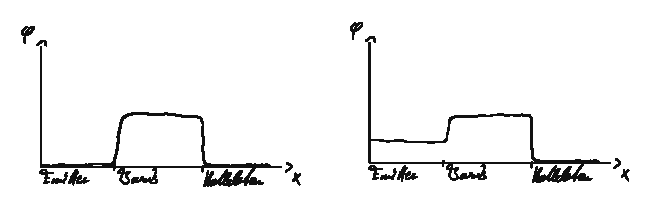
\includegraphics[width=0.9\textwidth]{A_crop.pdf}
        \caption[Potentialverlauf ohne und mit äußerer Spannung]{Potentialverlauf ohne (links) und mit (rechts) äußerer Spannung}
\end{figure}

\subsection{B}
Im Emitter ist eine hohe Elektronendichte; in der Basis ist nur eine geringe Löcherdichte; im Kollektor ist eine weniger starke Elektronendichte als im Emitter.

\subsection{C}
Es gilt 
\begin{align} 
        I_E&=I_B+I_C&\beta &=\diff[]{I_C}{I_B}&\alpha &=\diff[]{I_C}{I_E}&\gamma &=\diff[]{I_E}{I_B}
.\end{align} 
Leitet man nach $I_B$ ab folgt 
\begin{align} 
        &&\diff[]{I_E}{I_B}&=\diff[]{I_B}{I_B}+\diff[]{I_C}{I_B}&&\\
        \Leftrightarrow &&\gamma &=1+\beta .&&
\end{align} 
Leitet man nach $I_E$ ab folgt
\begin{align} 
        &&\diff[]{I_E}{I_E}&=\diff[]{I_B}{I_E}+\diff[]{I_C}{I_E}&&\\
        \Leftrightarrow &&1&=\dfrac{1}{\gamma }+\alpha &&\nonumber \\
        \Leftrightarrow &&\dfrac{1}{1-\alpha }&=\gamma &&\nonumber \\
        \Leftrightarrow &&\dfrac{1}{1-\alpha }-1&=\beta &&\nonumber \\
        \Leftrightarrow &&\dfrac{\alpha }{1-\alpha }&=\beta .&&
\end{align} 


\clearpage
\section{Auswertung}

\clearpage
\listoffigures
\listoftables
\bibliographystyle{plain}
\bibliography{refs}

%}}}

\end{document}

\include{Anhang.tex}

%}}}

\end{document}
